\documentclass{beamer}
\renewcommand\thesection{\arabic{section}}
\newcommand{\myfont}{\rmfamily\normalsize\upshape\mdseries}
\newcommand{\degree}{^\circ}
\title{\sffamily Review III(Slides 112 - 168)}
\subtitle{\textbf{Functions \& Sequence \& Convergence}\\ }
\institute[UM-SJTU JI]{University of Michigan-Shanghai Jiao Tong University Joint Institute}
\author{HamHam}
\usepackage{graphicx}
\usepackage{picinpar}
\usepackage{indentfirst}
\usepackage{chemformula}
\usepackage{geometry}
\usepackage{subfigure}
\usepackage{appendix}
\usepackage{amsfonts,amsmath,amssymb}
\usepackage{enumerate}
\usepackage{float}
\usepackage{geometry}
\usepackage{latexsym}
\usepackage{listings}
\usepackage{multicol,multirow,multido}
\usepackage{tabularx}
\usepackage{ulem}
\usepackage{tikz}
\usepackage{xcolor}
\usepackage{cite}
\usepackage{setspace}
\usepackage{hyperref}
\usepackage{textpos}
\usepackage{booktabs}

\usetheme[dove]{Boadilla}
\usecolortheme{dolphin}
\useoutertheme{miniframes}
\begin{document}
    \usebackgroundtemplate{\tikz\node[opacity=0.3]{
    
\includegraphics[width=\paperwidth,
    height=\paperheight]{hamster.jpg}
    };}
\begin{titlepage}
    \begin{center}
        VV186 - Honors Mathmatics II
    \end{center}
\end{titlepage}
\myfont
\section{Functions}
\begin{frame}
    \frametitle{Function}
\begin{center}   
    What is a function?\\
\end{center}
 There are some crucial properties should be mentioned when you want to describe a function, they are:
\begin{itemize}
    \item Domain:\\
        $dom\ f:=\{x\in X: (x,y)\ satisfies\ the\ requirement\ of\ f\}$
    \item Co-domain(target set): \\
        $Y=\{all\ "y"s\ such\ that\ (x,y)\ satisfies\ the\ requirement\ of\ f\}$
    \item Range:\\
        $ran\ f=\{y\ is\ in\ the\ target\ set:\ y=f(x)\}$
\end{itemize}
\begin{block}{Difference?}
    $~~f_1: \mathbb{R} \to \mathbb{R}, x \mapsto \sin x~~~~~~~~~~~~~~~~~~~~~~~~~~~~~~f_2: \mathbb{R} \to [-1,1], x \mapsto \sin x$
\end{block}
\end{frame}
\begin{frame}
    \frametitle{Function}
There are few ways to express a function:
\vspace{2em}
\begin{table}
    \centering
    \resizebox{11cm}{!}{%
    \begin{tabular}{cc}
        \toprule
        $Ways\ to\ express\ function$& $Comment$\\
        \midrule
        $f:X\rightarrow Y,x\mapsto f(x) $ & Pay attention to the forms of arrows.\\
        \\
        $f:X\rightarrow Y,f(x)=\dots $ & An intuitive way to express a function. \\
        \\
        $f=\{(x,y):P(x,y)\}$ & When hard to show the explicit form of $f$.\\
        \bottomrule
    \end{tabular}%
    }
\end{table}
\vspace{1em}
Comment: in \LaTeX, $\to$ is represented by $\backslash$to, while $\mapsto$ is $\backslash$mapsto
\end{frame}
\begin{frame}
    \frametitle{Implicit Function}
    The love formula:
    \begin{figure}
        \centering
        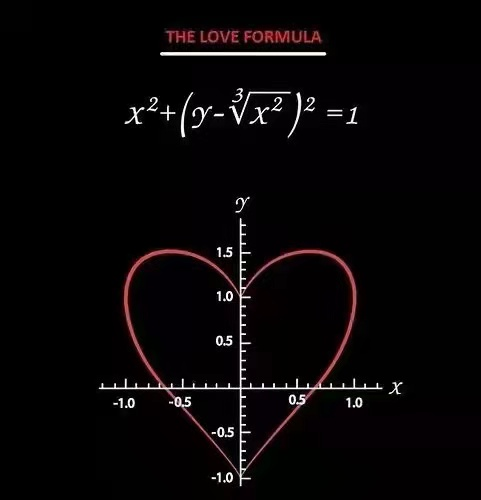
\includegraphics[width=0.42\textwidth]{implicit.jpg}
    \end{figure}
    Reference: \url{https://mp.weixin.qq.com/s/R1wLwediYMF5bKLlyTIDoA}
\end{frame}
\begin{frame}
    \frametitle{Function}
Common Misunderstanding:\\
\begin{center}
    Function is a \emph{graph}
\end{center}
\hspace{1em} Rather, one can view a function as a machine that sends each element in its domain to its target set. 
This is the passive view of function. The function is like an ''bow "that shoots an element in its domain to its 
target set. This is the active point view of a function.\\
\vspace{1em}
\hspace{1em} However, often it's intuitive (and useful) to express a function using graphs, especially when $f$ is an 
$\mathbb{R}$ to $\mathbb{R}$ function.\\
\hspace{15em}---comment from Zhang Leyang
\begin{figure}
    
\includegraphics[width=0.18\textwidth]{bow.png}
\end{figure}
\end{frame}
\begin{frame}
    \frametitle{Function}
Common Misunderstanding:\\
\begin{center}
    The \emph{co-domain is range} of $f$
\end{center}
\hspace{1em} The target set just contains $ran\ f$, it may be larger than $ran\ f$. For example, we can define a function 
\begin{equation*}
    g: \mathbb{R}\longmapsto \mathbb{R}, g(x)=x^2
\end{equation*}
\hspace{1em} The range of $f$ is $[0,+\infty)$, but the target set can simply be $\mathbb{R}$.\\
\vspace{3em}
Comment: On the contrary, the domain of $f$ contains exactly all the elements that have assignment with an element in 
$f$'s target set.
\end{frame}
\begin{frame}
    \frametitle{Function vs. Value}
    \vspace{1em}
    Consider a function 
    $$f : \Omega \rightarrow \mathbb{R}, x \mapsto f(x) $$
    What is $f$?
    \begin{itemize}
        \item $f$ is the function.
    \end{itemize}
    What is $f(x)$?
    \begin{itemize}
        \item $f(x)$ is the value of function at $x$.
    \end{itemize}
    What is $f(x_0)$?
    \begin{itemize}
        \item $f(x_0)$ is the value of function at $x_0$.
    \end{itemize}
\end{frame}

\section{Sequence}
\begin{frame}
    \frametitle{Sequence}
    Last year, a lot of students asked Prof. and TAs:
    \begin{itemize}
        \item Why is a sequence always have infinite items?
        \item What if a sequence only have finite items?
        \item ...
    \end{itemize}
    \pause
    
    \textcolor{red}{!!!}
	When we say “sequence” we usually assume that it is infinite.\\ 
    If it is finite, i.e., it contains only finite items
    , we usually say it is a “n-tuple”.
    Similarly, a subsequence of a sequence is infinite. 

\end{frame}
\begin{frame}
    \frametitle{Convergence \& Divergence}
    \begin{block}{Quick check:}
        \hspace{1em}
        \begin{itemize}
            \item A sequence is either convergent or divergent to (minus) infinity.
            \item A sequence is either convergent or divergent.
            \item If a sequence diverges, then it will go to (minus) infinity.
        \end{itemize}

    \end{block}
    \pause
    \hspace{1em}
    Of course, if a sequence is not convergent, 
    we say it is “divergent”. 
    However, it doesn’t mean it diverge to infinity. 
    An example is: $a_n=(-1)^n$. 

\end{frame}
\begin{frame}
    \frametitle{Important Results \& Theorem}
    \begin{itemize}
        \item A convergent sequence is bounded. (Slides 129)
        \item A convergent sequence has precisely one limit. (Slides 131)
        \item (\textbf{Squeeze Theorem}) \\Let $(a_n),(b_n)$ and $(c_n)$ be real sequences with $a_n<c_n<b_n$ 
            for sufficiently large $n\in\mathbb{N}$. Suppose that $\lim\ a_n=\lim\ b_n=:a$. Then 
            $(c_n)$ converges and $\lim\ c_n=a$. (Slide 134)\\
            \itshape{Comment:} It is extremely useful for examining the convergence of a sequence that is bounded.
        \myfont
        \item Let $(a_n)$ be a convergent sequence with limit $a$. Then any subsequence of $(a_n)$ 
            is convergent with the same limit. (Slide 146)
        \item Every real sequence has a monotonic subsequence. (Slide 147)
    \end{itemize}
    \vspace{1em}
    \textcolor{red}{Refer to slides, check the proofs on the weekend!}
\end{frame}
\begin{frame}
    \frametitle{Important Results \& Theorem}
    \begin{itemize}
        \item If a sequence has an accumulation point $x$, then there is a subsequence that converge to this point $x$. (Slides 150)
        \item (\textbf{Bolzano--Weierstraß})\\ Every bounded real sequence has an accumulation point. \\(Slide 151)\\
            \itshape{Comment.} There are at least two proofs, which we will discuss later.
        \item \myfont Every monotonic and bounded (real) sequence is convergent. (Slide 142)\\
            \itshape{Comment.} This result holds for sequence in any space with an ordering (otherwise it's 
            strange to even define ''monotonic").
    \end{itemize}
    \vspace{1em}
    \textcolor{red}{Refer to slides, check the proofs on the weekend!}
\end{frame}
\begin{frame}
    \frametitle{Bolzano--Weierstraß}
\textbf{Bolzano--Weierstraß} Every bounded real sequence has an accumulation point.
\begin{enumerate}
    \item Proof--1: On Horst's Slides.
    \item Proof--2:
        Since$(a_n)$ is bounded, assume $-M\leq a_n\leq M$ for all n. Divide the interval $[-M,M]$ into 2 sections:$[-M,0],[0,M]$.\\
        One of the interval, denoted by $I^{(1)}$, must contain infinitely many ''$a_n$"s(otherwise $(a_n)$is finite). Choose an $a_{(n,1)}$ 
        in $I^{(1)}$. We bisect $I^{(1)}$ into two intervals, one of which, denoted by $I^{(2)}$ must contain 
        infinitely many ''$a_n$ "s. Choose an $a_{(n,2)}$ in $I^{(2)}$ that is different from $a_{(n,1)}$ . By 
        repeatedly doing this procedure, we find a subsequence $(a_{n,k})_{k\in\mathbb{N}}$ that converges.
\end{enumerate}
\end{frame}
\begin{frame}
    \frametitle{Limit}
Some  results for limit.\\
\begin{center}
    Suppose $(a_n)\rightarrow a \in \mathbb{R}$ and $(b_n)\rightarrow b \in \mathbb{R}$  
\end{center}
\begin{enumerate}
    \item $\lim (a_n+b_n)=a+b$
    \item $\lim (a_n\cdot b_n) =a\cdot b$
    \item $\lim \frac{a_n}{b_n}=\frac{a}{b}, b\neq 0$
\end{enumerate}
We will prove 3 now.
\begin{block}{Danger:}
    \hspace{1em}
    $\lim (a_n+b_n)=\lim a_n + \lim b_n$?
\end{block}
\end{frame}
\begin{frame}
    \frametitle{Limit}
    \begin{center}
        $\lim \frac{a_n}{b_n}=\frac{a}{b}, b\neq 0$
    \end{center}
    Look at the definition and set your goal!
    \begin{block}{Goal:}
        \hspace{10em}
        $$\underset{\varepsilon>0}{\forall}~ \underset{N>0}{\exists} ~\underset{n>N}{\forall}~ |\frac{a_n}{b_n}-\frac{a}{b}|<\varepsilon$$
    \end{block}
    \textbf{Another approach:}\\
    \hspace{1em} Using the second result and try to prove $\lim \frac{1}{b_n}=\frac{1}{b}$
\end{frame}
\begin{frame}
    \frametitle{Proof}
    \hspace{1em} We want to prove that $|\frac{a_n}{b_n}-\frac{a}{b}|\rightarrow 0$ as $n\rightarrow \infty$.
    Since we don't want $b_n$ to be zero, we fix some $M\in \mathbb{N}$ such that $|b_n-b|<\frac{1}{2}|b|$ for 
    all $n>M$. Now, when $n>M$, we have:
    \begin{multline*}
        |\frac{a_n}{b_n}-\frac{a}{b}| 
    = |\frac{a_nb-b_na}{b_nb}|=|\frac{a_nb-ab+ab-b_na}{b_nb}| \\
     \leq \frac{|a_n-a||b|}{|b_nb|}+\frac{|a||b-b_n|}{|b_nb|} 
     <\frac{2|a_n-a||b|}{b^2}+\frac{2|a||b-b_n|}{b^2}
    \end{multline*}
    \hspace{1em} Given $\varepsilon >0$, choose $N>M$ such that 
\begin{equation*}
    \forall n> N, |a_n-a|<\frac{|b|\varepsilon}{4}|b_n-b|<\frac{b^2}{|a|}\cdot \frac{\varepsilon}{4}
\end{equation*} 
then we have:
\begin{equation*}
    \forall n>N, |\frac{a_n}{b_n}-\frac{a}{b}|<\frac{|b|\varepsilon}{4}\cdot\frac{2|b|}{b^2}+\frac{2|a|}{b^2}\cdot \frac{b^2}{|a|}\cdot \frac{\varepsilon}{4}<\varepsilon
\end{equation*}
\end{frame}
\section{Metric Space}
\begin{frame}
    \frametitle{Metric Space}
\begin{itemize}
    \item What is the definition of a metric?
    \item Why we want to introduce the idea of Metric Space?
    \item What new results can we explore from this new idea?
\end{itemize}
We want to generalize the idea of \textcolor{red}{convergence}, or close to some point. 
The most important thing is to define 
 the \textbf{Length Function}. Metric is just a \textcolor{blue}{nice} way of describing the 
 \textcolor{blue}{distance}.\\

\vspace{1em}
What properties a usual length function should have?
\begin{enumerate}
    \item Always positive.(distance)
    \item Symmetric.(distance)
    \item Followed \emph{Triangle Inequality}.(nice)
\end{enumerate}
\vspace{0.5em}
The remaining task is just 
transform these into mathematical language\dots
\end{frame}
\begin{frame}
    \frametitle{Metric Space}
A two variables functions 
$\rho(\cdot,\cdot):M\times M \rightarrow \mathbb{R}$
is called a metric if it satisfies:
\begin{enumerate}
    \item $\forall x,y\in M,\ \rho (x,y) \geq 0$ and $\rho (x,y)=0$ if and only if $x=y$.
    \item  $\forall x,y\in M,\ \rho (x,y)=\rho (y,x)$.
    \item  $\forall x,y,z\in M,\ \rho (x,z)\leq \rho (x,y)+\rho (y,z)$.
\end{enumerate}
\pause
Examples:
\begin{itemize}
    \item $M=\mathbb{R}^n$, the usual metric is given by 
        \begin{equation*}
            \rho ( (x_1,x_2,\dots,x_n), (y_1,y_2,\dots,y_n)) = \sqrt{\sum^{n}_{i=k}(x_i-y_i)^2 }
        \end{equation*} 
        and this is so-called \emph{Euclidean distance}.
    \item $M=\mathbb{N}, \rho(x,y)= \#\{ a:a\in [min\{x,y\},max\{x,y\}]\ \} $
    \item $M=\mathbb{R},\rho (x,y)=1 $ if $x\neq y$; $\rho (x,y)=0$ if $x=y$
\end{itemize}
\end{frame}
\begin{frame}
    \frametitle{Generalization of Convergence}
Then, by replacing the usual matric $\rho(x,y)=|x-y|$ and choosing our universal set $M$, we get the natural definition for
generalize convergence in metric space $(M,\rho)$ for a sequence $(a_n):\mathbb{N}\rightarrow M$, which is given by:
\begin{equation*}
    \lim_{n\rightarrow \infty}a_n=a\quad :\Leftrightarrow \quad \underset{\varepsilon>0}{\forall}\ \underset{N\in \mathbb{N}}{\exists}\ \underset{n>\mathbb{N}}{\forall} a_n\in B_\varepsilon(a)
\end{equation*}
where
\begin{equation*}
    B_\varepsilon(a)=\{ x\in M:\rho(x,a)<\varepsilon\},\quad \varepsilon>0,\quad a\in M.
\end{equation*}
\end{frame}
\begin{frame}
    \frametitle{Cauchy Sequences}
    A Sequence ($a_n$) in a metric space ($M$, $\rho$) is called a 
    \textbf{Cauchy Sequence} if
    $$\underset{\varepsilon>0}{\forall} ~\underset{N \in \mathbb{N}}{\exists}~\underset{m,n>N}{\forall} ~\rho(a_m,a_n)<\varepsilon$$ 
    An intuitive description of a Cauchy sequence is that the elements are
    getting closer together.\\
    \vspace{1em}
    \textcolor{red}{Some properties:}
    \begin{enumerate}
        \item Every Cauchy sequence is bounded.
        \item Every convergent sequence is Cauchy.
        \item But not every Cauchy sequence converges.
        \item If all Cauchy sequences in a metric space converges, 
        then the space is called \textbf{complete}.        
    \end{enumerate}
\end{frame}
\begin{frame}
    \frametitle{$\mathbb{C}$ is complete}
    In the lecture we have discussed that $\mathbb{R}$ is complete.
    For every Cauchy sequence ($z_n$) in $\mathbb{C}$, 
    we can write it into 2 real sequences ($x_n$) and ($y_n$)
     by writing $z_n = x_n + i \cdot  y_n$. Since 
    $$(x_m-x_n)^2\leq (x_m-x_n)^2+(y_m-y_n)^2=|z_m-z_n|^2<\varepsilon$$
    $$\Rightarrow |x_m-x_n|< \varepsilon$$
    and similar for ($y_n$), both ($x_n$) and ($y_n$) are Cauchy and thus convergent.
    Since a complex sequence converges if the real and imaginary parts
    converge, ($z_n$) converges and $\mathbb{C}$ is complete.

\end{frame}
\section{Exercises}
\begin{frame}
    \frametitle{Exercises}
    1$^*$. What's the difference between
    \begin{enumerate}
        \item Definition
        \item Proposition
        \item Theorem
        \item Lemma
        \item Corollary
    \end{enumerate}
    \vspace{2em}
    You can refer to 
    \url{https://blog.csdn.net/qq_38262728/article/details/111059766}
\end{frame}
\begin{frame}
    \frametitle{Exercises}
    2. Prove that $\lim_{n\rightarrow \infty} \sqrt[n]{n}=1$.\\ 
    \vspace{3em}
    Some results:
    \begin{itemize}
        \item $\lim_{n\rightarrow \infty} \sqrt[n]{a}=1,a>0$
        \item $\lim_{n\rightarrow \infty} \frac{1}{n^\alpha}=0,\alpha\in (0,+\infty)$
    \end{itemize}

\end{frame}
\begin{frame}
    \frametitle{Exercises}
    3. A sequence is defined as
    \begin{equation*}
        (S_n)_{n\in\mathbb{N}}, S_1=\sqrt{2}, S_2=\sqrt{2+\sqrt{2}}, S_3=\sqrt{2+\sqrt{2+\sqrt{2}}},...
    \end{equation*}
    Please prove that it is convergent and calculate the limit of $(S_n)$ as $n\rightarrow \infty$.
   
\end{frame}
\begin{frame}
    \frametitle{Exercises}
    4. Prove that every Cauchy sequence has at most one accumulation point.
    (A Former Midterm Question)
    
    \vspace{2em}
    Tips:
    \begin{itemize}
        \item You should work on an abstract metric space, using $\rho $ instead of $| \cdot |$.
        \item Try to prove this without using proof by contradiction!
    \end{itemize}
\end{frame}



\begin{frame}
    \frametitle{Exercises}
    5. Let ($a_n$) be a real sequence that converges to $L \in \mathbb{R}$.
    Prove that the sequence ($\frac{\sum_{i=1}^n a_i}{n}$) is convergent. 
    Furthermore $\underset{n\rightarrow \infty}{\lim} (\frac{\sum_{i=1}^n a_i}{n})=L $.
\end{frame}

\begin{frame}
    \frametitle{Exercises}
6. Let $(a_n),(b_n)$ be two real sequences. Furthermore, assume that $a_n<b_n$
for all $n$, $[a_{n+1}, b_{n+1}]\subseteq [a_n,b_n]$, $\lim (a_n-b_n)=0$. Prove that there 
is an unique $m\in [a_n,b_n]$ for all $n$, such that 
\begin{equation*}
    \lim a_n=\lim b_n=m
\end{equation*}
\end{frame}
\begin{frame}
    \frametitle{Exercises}
    7. Let ($a_n$) be a sequence that $a_n=\frac{1}{\sqrt{n^2+1}}+\cdots+\frac{1}{\sqrt{n^2+n}}$.
    Calculate the limit of ($a_n$).    

\end{frame}
\begin{frame}
    \frametitle{Reference}
    \begin{itemize}
        \item Exercises from 2019–Vv186 TA-Zhang Leyang.
        \item Exercises from 2020-Vv186 TA-Xia Yuxuan.
        \item Exercises from 2020-Vv186 TA-Hu Pingbang.
        \item The Love Formula, \url{https://mp.weixin.qq.com/s/R1wLwediYMF5bKLlyTIDoA}
        \item Mathematical Analysis I. \itshape School of Mathematical Sciences, ECNU,\myfont version 5. 
        Beijing: High Education Press, 2019.5 print.
    \end{itemize}

\end{frame}
\end{document}